\item \textbf{Try modeling the residuals as an AR process. Use the tools at your disposal to decide on an appropriate order and analyse the results. What is the impact of selecting different orders on the remaining residuals?}

\textit{For this question, we need to select the order of the \gls{AR} term (p). Therefore, \gls{PACF} and \gls{ACF} were plotted at first (see figure \ref{fig:Ass1_D1_PACF_ACF_X}).}  

\begin{figure}[H]
    \centering
    \begin{minipage}[b]{1\textwidth}
        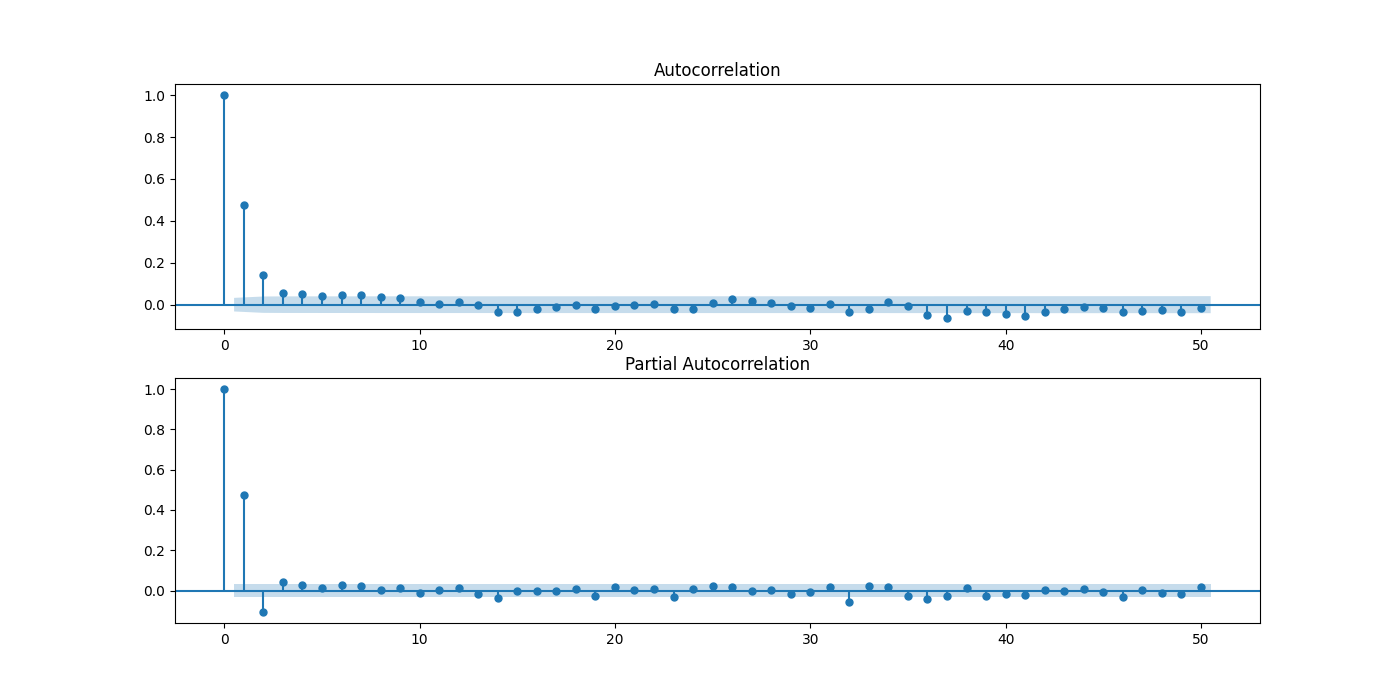
\includegraphics[width=\textwidth]{figures/Ass1/Ass1_D1_PACF_ACF_X.png}
    \end{minipage}
    \caption{A plot of the \gls{PACF} and \gls{ACF} of the residual part of the first dataset (residual of the STL method).}
    \label{fig:Ass1_D1_PACF_ACF_X}
\end{figure}

\textit{Sinse \gls{ACF} decaying (as figure \ref{fig:Ass1_D1_PACF_ACF_X} indicates), it can be concluded that the process is Auto Regressive. Also, based on PACF, the parameter of the \gls{AR} model should be start with an Auto Regressive model with lags 1 and 2 due to these two lags have a significant value.}



based on PACF we should start with an AR model with lags lags 1 ,2 ,10 ,13

so these are my starting points
must be stationary
these two plot do not tell us much


The PACF shows a single spike at the first lag and the ACF shows a tapering pattern. An AR(1) model is indicated.

2.How to find the order of the AR term (p)
\# PACF plot of 1st differenced series


You see how ACF is declining in amplitude exponentially, while PACF cuts off after lag 1. This may suggest that you\'re dealing with AR(1) process.

Note that the ACF shows exponential decay. This is indicative of a stationary series.

Note that the ACF shows an oscillation, indicative of a seasonal series. Note the peaks occur at lags of 12 months, 

The Akaike Information Critera (AIC) is a widely used measure of a statistical model. It basically quantifies 1) the goodness of fit, and 2) the simplicity/parsimony, of the model into a single statistic. When comparing two models, the one with the lower AIC is generally “better”.